\documentclass[aspectratio=169]{beamer}
\usepackage{tikz}
\usepackage{booktabs}
\usepackage{pifont}
\newcommand{\cmark}{\ding{51}}
\usepackage{array}
\usetikzlibrary{shapes.geometric, arrows.meta, positioning, fit, backgrounds, calc}

% Theme & Colors
\usetheme{Madrid}
\usecolortheme{default}
\definecolor{primary}{RGB}{6,90,130}
\definecolor{accent}{RGB}{2,195,154}
\definecolor{lightbg}{RGB}{240,248,255}

\setbeamercolor{frametitle}{bg=primary, fg=white}
\setbeamercolor{title}{fg=white}
\setbeamercolor{subtitle}{fg=accent}
\setbeamercolor{structure}{fg=primary}
\setbeamercolor{block title}{bg=primary, fg=white}
\setbeamercolor{block body}{bg=lightbg}
\setbeamerfont{frametitle}{size=\large, series=\bfseries}

\setbeamertemplate{navigation symbols}{}
\setbeamertemplate{footline}[frame number]

% Header with logo on every slide
\setbeamertemplate{headline}{
\begin{beamercolorbox}[wd=\paperwidth,ht=11.5ex,dp=1.5ex]{}
\hfill
\includegraphics[height=1cm]{images/chips_logo.png}
\hspace{0.3cm}
\end{beamercolorbox}
}

% TikZ Styles
\tikzset{
  block/.style={rectangle, rounded corners=4pt, draw=primary, thick,
                fill=lightbg, text width=2.2cm, align=center,
                minimum height=0.8cm, font=\small},
  arrow/.style={-{Stealth[length=6pt]}, thick, color=primary},
  highlight/.style={rectangle, rounded corners=4pt, draw=accent, very thick,
                    fill=accent!10, text width=2.2cm, align=center,
                    minimum height=0.8cm, font=\small\bfseries},
}

% Title Info
\title{Memory Controller for DDR Memories}
\author{
\textbf{Project Guide:} Prof. Mahesh A\\[0.3cm]
Pranav M -- PES2UG23EC076\\
Lalith -- PES2UG23EC074\\
Harshini -- PES2UG23EC058
}
\date{}

% ═══════════════════════════════════════════════════════════════════════════
\begin{document}

% Title Slide
\begin{frame}
  \titlepage
\end{frame}

% Slide 1: Introduction & Problem Statement
\begin{frame}{Introduction and Problem Statement}
  \textbf{What is a Memory Controller?}
  \begin{itemize}
    \item Bridge between processor/SoC and DRAM
    \item Manages read/write transactions, timing, refresh
    \item Critical for system performance and power
  \end{itemize}
  \vspace{0.5cm}
  \textbf{Our Goal:}\\
  Design and implement an RTL-level memory controller targeting DDR memories.
\end{frame}

% Slide 1b: Block Diagram (PNG from external)
\begin{frame}{System Block Diagram}
  \begin{center}
    \includegraphics[width=0.6\textwidth]{images/block_diagram.png}
  \end{center}
\end{frame}

% Memory Controller Slide 1: Evolution
\begin{frame}{Evolution of Memory Controller Placement}
  \begin{columns}
    \column{0.5\textwidth}
      \textbf{Northbridge-based Controller}
      \begin{itemize}
        \item Controller in external chipset
        \item Higher latency due to front-side bus
      \end{itemize}
      \vspace{0.3cm}
      \textbf{Integrated Memory Controller}
      \begin{itemize}
        \item Controller moves onto CPU/SoC die
        \item Simpler DRAM design, lower cost
        \item Advanced scheduling, prefetching, power management
      \end{itemize}

    \column{0.45\textwidth}
      \begin{center}
        \includegraphics[width=\textwidth]{images/memory_controller.png}
      \end{center}
  \end{columns}
\end{frame}

% Memory Controller Slide 2: DRAM Controller Functions
\begin{frame}{DRAM Controller Functions}
  \begin{columns}
    \column{0.5\textwidth}
      \textbf{Correct Operation}
      \begin{itemize}
        \item Ensure refresh and timing constraints
        \item Translate requests to DRAM commands
      \end{itemize}
      \vspace{0.2cm}
      \textbf{Performance}
      \begin{itemize}
        \item Schedule requests for high throughput
        \item Reordering and row-buffer management
      \end{itemize}
      \vspace{0.2cm}
      \textbf{Power Management}
      \begin{itemize}
        \item Manage DRAM power modes and thermals
      \end{itemize}

    \column{0.45\textwidth}
      \begin{block}{Why Complex Controllers?}
        \scriptsize
        \begin{itemize}
          \item Reduces DRAM die area and DIMM cost
          \item Centralizes protocol changes
          \item Improves scalability across generations
          \item Better performance-per-watt
        \end{itemize}
      \end{block}
  \end{columns}
\end{frame}

% Memory Controller Slide 3: Timing Constraints
\begin{frame}{Challenge -- Many DRAM Timing Constraints}
  \textbf{DRAM has 50+ timing constraints that must be obeyed. Key examples:}
  \vspace{0.2cm}
  \begin{columns}
    \column{0.55\textwidth}
      \begin{block}{}
        \scriptsize
        \begin{tabular}{lp{5cm}}
          \toprule
          \textbf{Constraint} & \textbf{Description} \\
          \midrule
          tWTR & Min cycles before READ after WRITE \\
          tRC  & Min cycles between consecutive ACTIVATEs to same bank \\
          tRRD & Min cycles between ACTIVATEs to different banks \\
          tFAW & Max 4 ACTIVATEs in a rolling time window \\
          \bottomrule
        \end{tabular}
      \end{block}

    \column{0.4\textwidth}
      \textbf{Controller must track:}
      \begin{itemize}
        \item Channels, banks, ranks
        \item Data bus, address bus
        \item Row buffers
        \item Refresh intervals
        \item Power states
      \end{itemize}
  \end{columns}
\end{frame}

% Slide 2: SDR vs DDR
\begin{frame}{SDR vs DDR -- What Changed?}
  \begin{columns}
    \column{0.52\textwidth}
      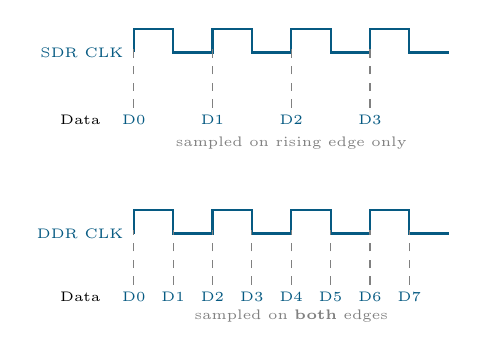
\begin{tikzpicture}
        % SDR CLK
        \draw[thick, primary] (0,5.8) node[left,font=\tiny]{SDR CLK}
          -- (0,6.1) -- (0.5,6.1) -- (0.5,5.8)
          -- (1.0,5.8) -- (1.0,6.1) -- (1.5,6.1) -- (1.5,5.8)
          -- (2.0,5.8) -- (2.0,6.1) -- (2.5,6.1) -- (2.5,5.8)
          -- (3.0,5.8) -- (3.0,6.1) -- (3.5,6.1) -- (3.5,5.8) -- (4.0,5.8);
        \node[left, font=\tiny] at (-0.3,4.95) {Data};
        \foreach \x/\lbl in {0/D0, 1.0/D1, 2.0/D2, 3.0/D3}{
          \draw[dashed, gray, thin] (\x,5.1) -- (\x,5.85);
          \node[font=\tiny, color=primary] at (\x,4.95) {\lbl};
        }
        \node[font=\tiny, color=gray] at (2.0,4.65) {sampled on rising edge only};

        % DDR CLK
        \draw[thick, primary] (0,3.5) node[left,font=\tiny]{DDR CLK}
          -- (0,3.8) -- (0.5,3.8) -- (0.5,3.5)
          -- (1.0,3.5) -- (1.0,3.8) -- (1.5,3.8) -- (1.5,3.5)
          -- (2.0,3.5) -- (2.0,3.8) -- (2.5,3.8) -- (2.5,3.5)
          -- (3.0,3.5) -- (3.0,3.8) -- (3.5,3.8) -- (3.5,3.5) -- (4.0,3.5);
        \node[left, font=\tiny] at (-0.3,2.7) {Data};
        \foreach \i/\lbl in {0/D0,1/D1,2/D2,3/D3,4/D4,5/D5,6/D6,7/D7}{
          \draw[dashed, gray, thin] (0.5*\i,2.85) -- (0.5*\i,3.55);
          \node[font=\tiny, color=primary] at (0.5*\i,2.7) {\lbl};
        }
        \node[font=\tiny, color=gray] at (2.0,2.45) {sampled on \textbf{both} edges};

      \end{tikzpicture}

    \column{0.4\textwidth}
      \begin{block}{Key Differences}
        \scriptsize
        \begin{tabular}{lll}
          \toprule
          & \textbf{SDR} & \textbf{DDR} \\
          \midrule
          Transfer & Rising edge & Both edges \\
          Bandwidth & 1$\times$ & 2$\times$ \\
          Voltage & 3.3V & 2.5V / lower \\
          Prefetch & 1n & 2n \\
          \bottomrule
        \end{tabular}
      \end{block}
  \end{columns}
\end{frame}

% Slide 3: DDR Generations
\begin{frame}{DDR Generations -- Evolution}
  \begin{center}
  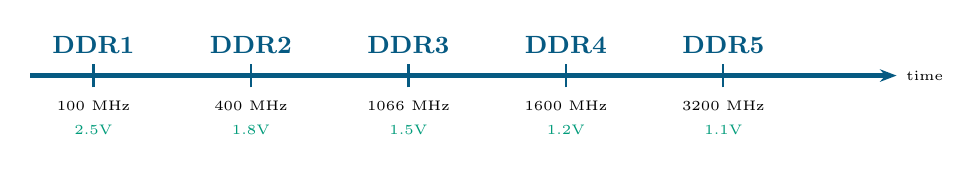
\begin{tikzpicture}[node distance=0.0cm]
    \draw[arrow, line width=2pt] (0,0) -- (11,0);

    \foreach \x/\gen/\speed/\volt in {
      0.8/DDR1/100 MHz/2.5V,
      2.8/DDR2/400 MHz/1.8V,
      4.8/DDR3/1066 MHz/1.5V,
      6.8/DDR4/1600 MHz/1.2V,
      8.8/DDR5/3200 MHz/1.1V}{
      \draw[thick, primary] (\x, -0.15) -- (\x, 0.15);
      \node[above, font=\small\bfseries, color=primary] at (\x, 0.15) {\gen};
      \node[below, font=\tiny] at (\x, -0.2) {\speed};
      \node[below, font=\tiny, color=accent!80!black] at (\x, -0.5) {\volt};
    }

    \node[right, font=\tiny] at (11, 0) {time};
  \end{tikzpicture}
  \end{center}

  \vspace{0.4cm}
  \textbf{Each generation brought:}
  \begin{itemize}
    \item Higher clock frequencies and bandwidth
    \item Lower operating voltage (power savings)
    \item Improved prefetch depth (2n $\to$ 4n $\to$ 8n $\to$ 16n)
    \item Key challenges as speeds increase: signal integrity, timing closure, power delivery, and clock domain crossing
  \end{itemize}
\end{frame}

% DDR Timing Diagram 1: Write
\begin{frame}{DDR Timing -- Write}
  \begin{center}
    \includegraphics[width=0.92\textwidth]{images/ddr_write.png}
  \end{center}
\end{frame}

% DDR Timing Diagram 2: Read
\begin{frame}{DDR Timing -- Read}
  \begin{center}
    \includegraphics[width=0.8\textwidth]{images/ddr_read.png}
  \end{center}
\end{frame}

% DDR Timing Diagram 3: Read Burst
\begin{frame}{DDR Timing -- Read Burst}
  \begin{center}
    \includegraphics[width=0.92\textwidth]{images/ddr_read_burst.png}
  \end{center}
\end{frame}

% Slide 4: LPDDR
\begin{frame}{LPDDR -- Low Power DDR}
  \begin{columns}
    \column{0.5\textwidth}
      \textbf{Requirements}
      \begin{itemize}
        \item High bandwidth
        \item Low latency
        \item Power efficient
      \end{itemize}
      \vspace{0.4cm}
      \textbf{Advanced Power Management}
      \begin{itemize}
        \item Partial Array Self Refresh (PASR)
        \item Temperature Compensated Self Refresh (TCSR)
        \item Deep Power-Down (DPD)
      \end{itemize}

    \column{0.45\textwidth}
      \begin{block}{LPDDR vs DDR}
        \scriptsize
        \begin{tabular}{lll}
          \toprule
          & \textbf{DDR5} & \textbf{LPDDR5} \\
          \midrule
          Voltage & 1.1V & 1.05V \\
          Form factor & DIMM & PoP/BGA \\
          Power modes & Basic & PASR/TCSR/DPD \\
          \bottomrule
        \end{tabular}
      \end{block}
  \end{columns}
\end{frame}


% Slide 5: Async FIFO -- Functionality
\begin{frame}{Asynchronous FIFO -- Functionality}
  \begin{columns}
    \column{0.48\textwidth}
      \textbf{Clock Domain Crossing (CDC)}
      \begin{itemize}
        \item AXI clock $\neq$ PHY/memory clock
        \item Direct signal passing causes metastability
        \item Async FIFO safely bridges the two domains
      \end{itemize}
      \vspace{0.3cm}
      \textbf{Our Implementation}
      \begin{itemize}
        \item Parameterizable depth and width
        \item Gray-coded pointers for safe CDC
        \item 2-FF synchronizer (\texttt{cdc\_sync}) module
        \item Credit-based flow control
      \end{itemize}

    \column{0.48\textwidth}
      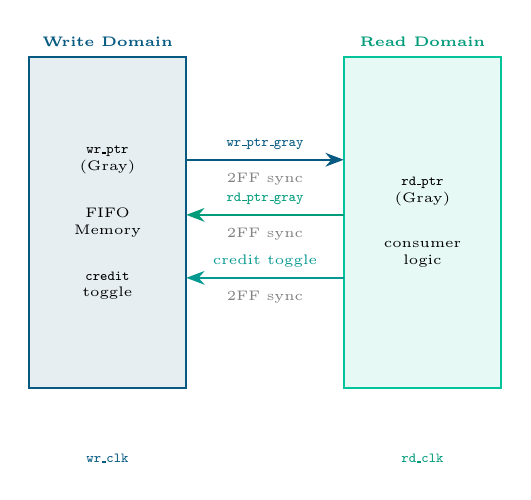
\begin{tikzpicture}[node distance=0.5cm]
        % Write domain box
        \node[rectangle, draw=primary, thick, fill=primary!10,
              minimum width=2.0cm, minimum height=4.2cm,
              label={[font=\tiny\bfseries, color=primary]above:Write Domain}]
              (wd) at (0,0) {};
        \node[font=\tiny, align=center] at (0, 0.8) {\texttt{wr\_ptr}\\(Gray)};
        \node[font=\tiny, align=center] at (0, 0.0) {FIFO\\Memory};
        \node[font=\tiny, align=center] at (0,-0.8) {\texttt{credit}\\toggle};

        % Read domain box
        \node[rectangle, draw=accent, thick, fill=accent!10,
              minimum width=2.0cm, minimum height=4.2cm,
              label={[font=\tiny\bfseries, color=accent!80!black]above:Read Domain}]
              (rd) at (4.0,0) {};
        \node[font=\tiny, align=center] at (4.0, 0.4) {\texttt{rd\_ptr}\\(Gray)};
        \node[font=\tiny, align=center] at (4.0,-0.4) {consumer\\logic};

        % Path 1: wr_ptr → rd domain
        \draw[-{Stealth}, thick, color=primary]
          (1.0, 0.8) -- (3.0, 0.8)
          node[midway, above, font=\tiny]{\texttt{wr\_ptr\_gray}};
        \node[font=\tiny, color=gray] at (2.0, 0.55) {2FF sync};

        % Path 2: rd_ptr → wr domain
        \draw[-{Stealth}, thick, color=accent!80!black]
          (3.0, 0.1) -- (1.0, 0.1)
          node[midway, above, font=\tiny]{\texttt{rd\_ptr\_gray}};
        \node[font=\tiny, color=gray] at (2.0,-0.15) {2FF sync};

        % Path 3: credit toggle → wr domain
        \draw[-{Stealth}, thick, color=accent!60!primary]
          (3.0,-0.7) -- (1.0,-0.7)
          node[midway, above, font=\tiny]{credit toggle};
        \node[font=\tiny, color=gray] at (2.0,-0.95) {2FF sync};

        % Clock labels at bottom
        \node[font=\tiny, color=primary, below=0.7cm of wd] {\texttt{wr\_clk}};
        \node[font=\tiny, color=accent!80!black, below=0.7cm of rd] {\texttt{rd\_clk}};
      \end{tikzpicture}
  \end{columns}
\end{frame}

% Slide 6: Async FIFO -- Block Diagram
\begin{frame}{Asynchronous FIFO -- Block Diagram}
  \begin{center}
    \includegraphics[width=0.85\textwidth]{images/fifo_block.png}
  \end{center}
\end{frame}

% Slide 7: AXI -- Overview
\begin{frame}{AXI Interface -- Overview}
  \begin{columns}
    \column{0.45\textwidth}
      \textbf{Why AXI?}
      \begin{itemize}
        \item Industry standard (ARM AMBA)
        \item Separate read and write channels
        \item Burst transfers, out-of-order support
        \item Decouples master from slave
      \end{itemize}
      \vspace{0.2cm}
      \textbf{5 Channels:}
      \begin{itemize}
        \item AW -- Write Address
        \item W -- Write Data
        \item B -- Write Response
        \item AR -- Read Address
        \item R -- Read Data
      \end{itemize}

    \column{0.5\textwidth}
      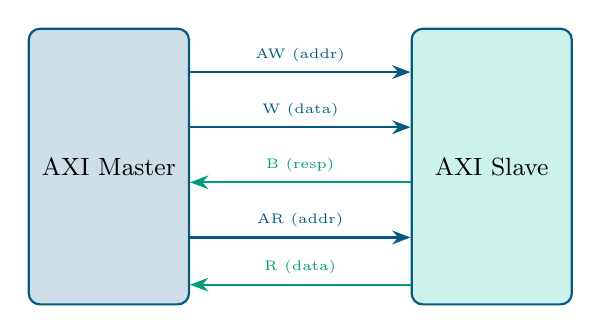
\begin{tikzpicture}[node distance=0.3cm and 1.5cm]
        \node[block, fill=primary!20, minimum height=3.5cm, text width=1.8cm]
          (master) {AXI Master};
        \node[block, fill=accent!20, minimum height=3.5cm, text width=1.8cm,
              right=2.8cm of master] (slave) {AXI Slave};

        % Write channels
        \foreach \y/\ch in {1.2/AW (addr), 0.5/W (data)}{
          \draw[-{Stealth}, thick, color=primary]
            ($(master.east)+(0,\y)$) -- ($(slave.west)+(0,\y)$)
            node[midway, above, font=\tiny]{\ch};
        }
        \draw[-{Stealth}, thick, color=accent!80!black]
          ($(slave.west)+(0,-0.2)$) -- ($(master.east)+(0,-0.2)$)
          node[midway, above, font=\tiny]{B (resp)};
        % Read channels
        \draw[-{Stealth}, thick, color=primary]
          ($(master.east)+(0,-0.9)$) -- ($(slave.west)+(0,-0.9)$)
          node[midway, above, font=\tiny]{AR (addr)};
        \draw[-{Stealth}, thick, color=accent!80!black]
          ($(slave.west)+(0,-1.5)$) -- ($(master.east)+(0,-1.5)$)
          node[midway, above, font=\tiny]{R (data)};
      \end{tikzpicture}
  \end{columns}
\end{frame}

% Slide 8: AXI -- Transaction Flow
\begin{frame}{AXI -- Write and Read Transaction Flow}
  \begin{columns}
    \column{0.48\textwidth}
      \textbf{Write Transaction}
      \begin{center}
      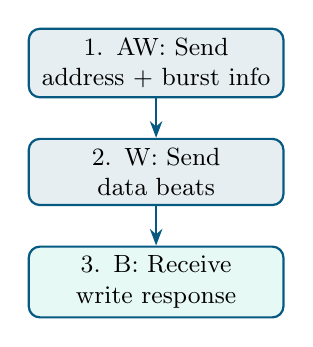
\begin{tikzpicture}[node distance=0.5cm]
        \node[block, fill=primary!10, text width=3cm] (aw) {1. AW: Send address + burst info};
        \node[block, below=of aw, fill=primary!10, text width=3cm] (w)  {2. W: Send data beats};
        \node[block, below=of w,  fill=accent!10,  text width=3cm] (b)  {3. B: Receive write response};
        \draw[arrow] (aw) -- (w);
        \draw[arrow] (w)  -- (b);
      \end{tikzpicture}
      \end{center}

    \column{0.48\textwidth}
      \textbf{Read Transaction}
      \begin{center}
      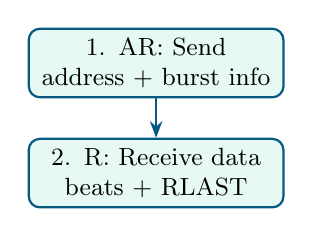
\begin{tikzpicture}[node distance=0.5cm]
        \node[block, fill=accent!10, text width=3cm] (ar) {1. AR: Send address + burst info};
        \node[block, below=of ar, fill=accent!10, text width=3cm] (r)  {2. R: Receive data beats + RLAST};
        \draw[arrow] (ar) -- (r);
      \end{tikzpicture}
      \end{center}
      \vspace{0.5cm}
      \textbf{Handshake:} Every channel uses \texttt{VALID}/\texttt{READY} handshake -- transfer occurs only when both are high.
  \end{columns}
\end{frame}

% Slide 8b: Why AXI is Perfect for DDR
\begin{frame}{Why AXI is Perfect for DDR Memory Controllers}
  \begin{center}
  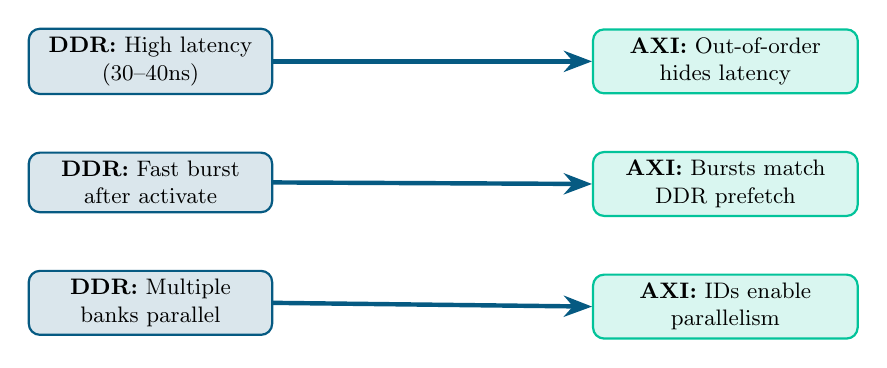
\begin{tikzpicture}[node distance=0.8cm, scale=0.9, every node/.style={transform shape}]
    \node[rectangle, rounded corners=4pt, draw=primary, thick, fill=primary!15,
          text width=3.2cm, align=center, font=\small] (lat)
          {\textbf{DDR:} High latency\\(30--40ns)};
    \node[below=of lat, rectangle, rounded corners=4pt, draw=primary, thick,
          fill=primary!15, text width=3.2cm, align=center, font=\small] (burst)
          {\textbf{DDR:} Fast burst\\after activate};
    \node[below=of burst, rectangle, rounded corners=4pt, draw=primary, thick,
          fill=primary!15, text width=3.2cm, align=center, font=\small] (bank)
          {\textbf{DDR:} Multiple\\banks parallel};

    \node[right=4.5cm of lat, rectangle, rounded corners=4pt, draw=accent, thick,
          fill=accent!15, text width=3.5cm, align=center, font=\small] (sol1)
          {\textbf{AXI:} Out-of-order\\hides latency};
    \node[below=of sol1, rectangle, rounded corners=4pt, draw=accent, thick,
          fill=accent!15, text width=3.5cm, align=center, font=\small] (sol2)
          {\textbf{AXI:} Bursts match\\DDR prefetch};
    \node[below=of sol2, rectangle, rounded corners=4pt, draw=accent, thick,
          fill=accent!15, text width=3.5cm, align=center, font=\small] (sol3)
          {\textbf{AXI:} IDs enable\\parallelism};

    \draw[-{Stealth}, ultra thick, color=primary] (lat.east) -- (sol1.west);
    \draw[-{Stealth}, ultra thick, color=primary] (burst.east) -- (sol2.west);
    \draw[-{Stealth}, ultra thick, color=primary] (bank.east) -- (sol3.west);
  \end{tikzpicture}
  \end{center}
  \vspace{0.2cm}
  \begin{center}
    \textcolor{primary}{\textbf{Perfect match between protocol and memory!}}
  \end{center}
\end{frame}
\begin{frame}{PHY Layer -- Physical Interface}
  \begin{columns}
    \column{0.5\textwidth}
      \textbf{Role of PHY}
      \begin{itemize}
        \item Bridge between the memory controller and the memory
        \item Temporarily stores instructions and data in buffers
        \item Performs Write Leveling, DQS Gate Training and Vref Training
      \end{itemize}

    \column{0.45\textwidth}
      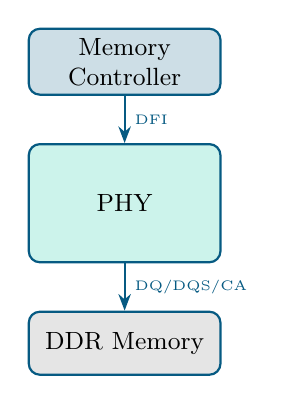
\begin{tikzpicture}[node distance=0.6cm]
        \node[block, fill=primary!20, text width=2.2cm] (ctrl) {Memory\\Controller};
        \node[block, below=of ctrl, fill=accent!20, text width=2.2cm,
              minimum height=1.5cm] (phy) {PHY};
        \node[block, below=of phy, fill=gray!20, text width=2.2cm] (ddr) {DDR Memory};
        \draw[arrow] (ctrl) -- (phy) node[midway, right, font=\tiny]{DFI};
        \draw[arrow] (phy) -- (ddr) node[midway, right, font=\tiny]{DQ/DQS/CA};
      \end{tikzpicture}
  \end{columns}
\end{frame}

% Slide 10: DFI Interface
\begin{frame}{DFI Interface}
  \begin{columns}
    \column{0.55\textwidth}
      \textbf{What is DFI?}
      \begin{itemize}
        \item Universal language for PHY interoperability
        \item Decouples memory controller from PHY implementation
      \end{itemize}
      \vspace{0.4cm}
      \textbf{Three Pillars of DFI 5.0/5.1}
      \begin{itemize}
        \item PHY independent boot sequence
        \item Expanding frequency range support
        \item New PHY-to-Controller Interface interaction
      \end{itemize}

    \column{0.4\textwidth}
      \begin{center}
        \includegraphics[width=0.8\textwidth]{images/ddr_phy.png}
      \end{center}
  \end{columns}
\end{frame}

% Slide 11: Next Steps
\begin{frame}{Next Steps}
  \begin{center}
  \vspace{1cm}
  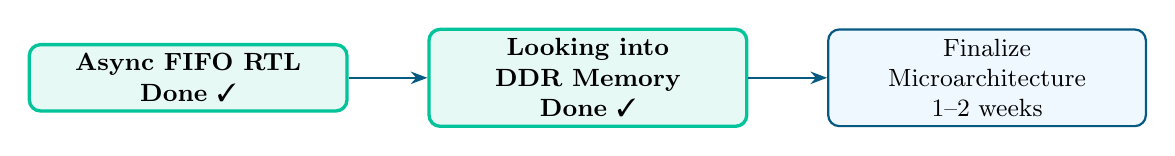
\begin{tikzpicture}
    \node[highlight, text width=3.8cm] (s1) {Async FIFO RTL\\{\small Done \cmark}};
    \node[highlight, right=1cm of s1, text width=3.8cm] (s2) {Looking into DDR Memory\\{\small Done \cmark}};
    \node[block, right=1cm of s2, text width=3.8cm] (s3) {Finalize\\Microarchitecture\\{\small 1--2 weeks}};
    \draw[arrow] (s1) -- (s2);
    \draw[arrow] (s2) -- (s3);
  \end{tikzpicture}
  \end{center}
\end{frame}

\end{document}